\newpage
\section{Mission 3: Herding chaos}\label{sec:mission3}

\begin{minipage}{0.45\linewidth}
Due to political differences, and in spite of the colony assembly's best efforts, each base in the planet adopted a different LAN technology (!).
Even though communications are satisfactory within each base, at the moment it is impossible to directly connect any two computers from two different bases.
%
Once again, the colony is asking for your help.\\
\end{minipage}
\hspace{0.04\linewidth}
\begin{minipage}{0.5\linewidth}
\vspace{-1cm}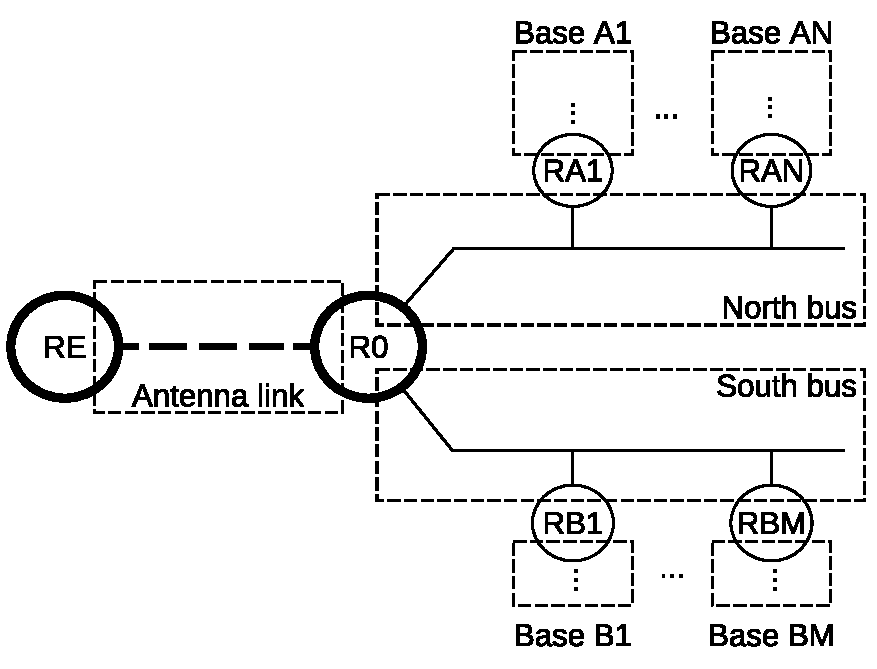
\includegraphics[width=\linewidth]{colony_network_map.pdf}
\end{minipage}

\noindent
Thanks to everyone's sacrifices, the colony is now in a position to build and install a new router and two cabled buses.
These are represented with a thicker line in the diagram below.
%
% \noindent
Your long-term goal is to make it possible to have internetwork communications between any two nodes of any two bases.
For now, you will be designing the physical and logical infrastructure.\\

\subsection*{Report details}

All the bases employ the IPv4 protocol, and there are multiple bases connected to both the North and the South buses.
Each base contains a single LAN. Coordinate with others so that \textit{no two LANs have the same size}.

\begin{enumerate}[itemsep=0.25cm]
\item Within your group:
\begin{itemize}[itemsep=0.25cm]
    \item Determine how many addresses you need so that each device can uniquely identified within your LAN.
    Choose the minimum LAN size that can satisfy this requirement, and quantify the free ``space'' available in
    your LAN.
    \item Indicate how many of the 32~bits of an IPv4 address you need to identify a single device connected to your base LAN.
    What concept used in IP is most closely related to this number? How can this structure be useful?\\[0.2cm]
\end{itemize}

\begin{center}
\begin{bytefield}{18}
\bitbox{8}{Network ID} & \bitbox{15}{Host ID}\\
\end{bytefield}
\end{center}

\item In coordination with the other groups in the classroom:
\begin{itemize}[itemsep=0.25cm]
\item Create a LAN for the North Bus, and describe all physical and logical addresses connected to it.
\item Ensure that the IPv4 address blocks assigned to the LANs are of different size and do not overlap.
\item Using the blackboard or a shared document, list all LANs, their sizes and (updated) address ranges.
\end{itemize}

\end{enumerate}

\subsection*{Feedback details}

Use a similar feedback process as in the previous missions, making sure to touch on:

\begin{enumerate}[itemsep=0.25cm]
\item Are the LANs correctly dimensioned?
\item Is there any collision between the blocks?
\item Did the original report extract all information about the IP address structure?
\end{enumerate}
